\documentclass[11pt]{article}
\usepackage[final]{acl2023}
\usepackage{times}
\usepackage{latexsym}
\usepackage{amsmath,amssymb,booktabs,graphicx,float,placeins}
\usepackage{colortbl}
\usepackage[T1]{fontenc}
\usepackage[utf8]{inputenc}
\usepackage{microtype}
\title{Talk Like a Structured Graph? Structural Statistics Help Small LLMs\\Mainly by Stating the Answer}
\author{
  Inbal Moryles\\
  \footnotesize\texttt{github.com/iinbal}\\
  \footnotesize\texttt{inbalmoryles@tau.ac.il}
  \And
  Gal Barak\\
  \footnotesize\texttt{github.com/GalBrk}\\
  \footnotesize\texttt{galbarak2@mail.tau.ac.il}
  \And
  Nitzan Zacharia\\
  \footnotesize\texttt{github.com/NitzanZacharia}\\
  \footnotesize\texttt{zacharia1@mail.tau.ac.il}
}
\date{}
\begin{document}
\raggedbottom
\maketitle
\begin{abstract}
Do structural encodings that help graph neural networks help a language model read a graph as text? We state degree, clustering and random-walk returns as a primer before GraphQA's incident encoding, and test Qwen3-1.7B and Qwen3-4B, thinking off and on, on paired graphs. Stated degrees give the clearest effects, in both directions: node-degree accuracy rises by $7.5$--$12.2$ points where the model's own count is unreliable and falls by $6.5$--$8.0$ where it is reliable. Clustering and RWSE state no answer; their effects are mostly small, change sign with task and model, and never significantly improve reading the queried node's edges. A near-constant component-count sentence does for plain Qwen3-4B, which then restates that node's line far more often. Checked against the graph, correct cycle answers can rest on nonexistent edges. Structural statistics help small models mainly by stating the answer, not by improving how they compute it.\footnote{\url{https://github.com/GalBrk/GraphTalk}} % [main] [joint] [comp] [compproc] [ccanswer]
\end{abstract}

\section{Introduction}
\label{sec:intro}
Degree and random-walk encodings help graph models \citep{dwivedi2022graph,rampasek2022recipe}. A language model reading a textual graph must instead recover such quantities itself, with accuracy sensitive to the encoding \citep{fatemi2023talklikeagraph,wang2023nlgraph}. We ask: \emph{when a frozen language model reads a textual graph, do explicit structural statistics improve execution of graph queries?} Here execution means deriving an answer from edges rather than copying it from a primer (\S\ref{sec:method}).

A primer can supply an answer, offer a clue, or alter how graph text is used. In an independent-edge graph every edge is independent of the others, so clustering and return probabilities carry little information about GraphQA's answers beyond what they reveal of degrees and density (\S\ref{sec:states}); a gain from them mostly reflects how the model reads the prompt. We compare it with a graph-blind solver, a structure-free \emph{filler}, and the same model's thinking mode, which for Qwen3-1.7B uses $6.2$--$17.1$ times as many output tokens on node degree. Degree, which supplies the queried value and the terms for edge count, is the positive control. % [ddgap]

\paragraph{Contributions.} (i) A stated answer substitutes for execution: it helps where the model's own count is unreliable and hurts plain Qwen3-4B where its count is reliable, while still helping the other arms at matched accuracy (\S\ref{sec:readoff}). (ii) Other statistics have mostly small effects whose sign depends on the model (\S\ref{sec:side}). (iii) A near-constant sentence that changes plain Qwen3-4B's procedure matches thinking on one task, and filler moves the same procedure the other way (\S\ref{sec:side}, \S\ref{sec:vsthink}). (iv) Responses show stated values being used but not other statistics (\S\ref{sec:reston}).

\section{Related Work}
\label{sec:related}
\paragraph{Graphs as text.} GraphQA \citep{fatemi2023talklikeagraph} and NLGraph \citep{wang2023nlgraph} show that accuracy depends on encoding, task and graph structure; NLGraph's build-a-graph prompts also change the procedure by instruction. Learned structural tokens raise GraphQA accuracy \citep{perozzi2024letyourgraph}, and prompts have carried motif descriptions \citep{das2024modality}, but structure written into a prompt tends to be read as context rather than as topology \citep{huang2024can}. We keep GraphQA's encoding and tasks and add only a preamble of graph-learning statistics.

\paragraph{Controls and responses.} Irrelevant text, input length and formatting change answers \citep{shi2023distracted,levy2024sametask,sclar2024quantifying}, so we compare against a structure-free filler. Explanations need not reflect the computation behind them \citep{turpin2023unfaithful}, so we check every graph claim a response makes against the graph.

\section{Method}
\label{sec:method}
\paragraph{Models and graphs.} Qwen3-1.7B and Qwen3-4B \citep{qwen2025qwen3}, each with thinking off and on, make four \emph{arms} (1.7P, 1.7T, 4P, 4T in tables). Decoding is zero-shot and greedy, one response per prompt (budgets in Appendix~\ref{app:audit}). A pilot on the published GraphQA graphs with Gemma~4 \citep{gemma4} and Qwen3-8B/14B left most arms near ceiling (Appendix~\ref{app:pilot}), and even at $40$ nodes Qwen3-8B answers nearly every node-degree query correctly ($96.5$--$99.8\%$). We therefore use harder graphs and smaller models, so that accuracy without a primer leaves room to measure a change in either direction. Our independent-edge $G(n,p)$ graphs \citep{gilbert1959random} have $n=40$ at four edge densities up to $p=.50$ (the \emph{main sweep}) and, for node degree and edge existence, three more up to $p=.85$. Every condition and arm sees the same $100$ graphs per task and density, so every comparison is paired. % [setup] [fixdeg8]

\begin{figure}[!t]
\centering
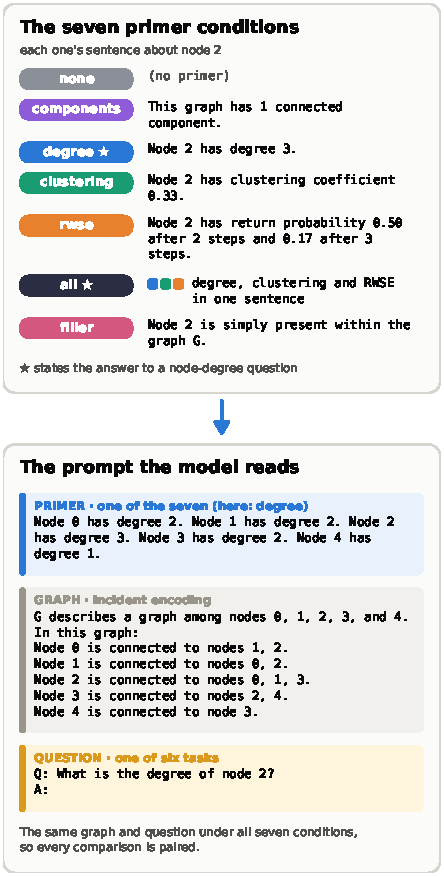
\includegraphics[width=0.82\columnwidth]{fig_primer_usage.pdf}
\caption{How a primer is used. Top: the seven conditions, each with its sentence about node~2 of a five-node example (the study's graphs have $40$ nodes); $\bigstar$ marks the two that state a node-degree answer. Bottom: the prompt the model reads, one primer followed by GraphQA's incident encoding and the question.}
\label{fig:prompt}
\end{figure}

\paragraph{Tasks.} GraphQA's six tasks in its incident encoding (Figure~\ref{fig:prompt}). Four have answers that vary: node degree, connected nodes (the queried node's neighbors, exact set match), edge count and edge existence. Node count (always $40$) and cycle check (always yes) have constant answers here (Appendix~\ref{app:more}); cycle check serves only to ask what correct answers rest on. % [setup]

\paragraph{Primers and controls.} Before the encoding we place no primer, one sentence per node giving its degree, local clustering coefficient or return probabilities after 2 and 3 steps (a truncated RWSE; \citealp{dwivedi2022graph}), or \emph{all} three (Appendix~\ref{app:audit}). Two diagnostics are a short sentence giving the number of connected components, and a filler that names every node but gives no graph statistic. The filler is about as long as clustering, longer than degree and shorter than RWSE and all three (Appendix Table~\ref{tab:primerlength}). The graph-blind solver answers from primer text alone.

\begin{table*}[t]
\centering\scriptsize
\setlength{\tabcolsep}{3.4pt}
\begin{tabular}{llrrrrrrr}
\toprule
Task & Arm & none & degree & clustering & RWSE & all & components & filler\\
\midrule
Degree & 1.7P & 60.50 & \cellcolor{black!12}$\mathbf{+7.5}^{\mathrm{f}}$ & $+3.0$ & $+4.0$ & \cellcolor{black!12}$\mathbf{+10.2}^{\mathrm{f}}$ & $+1.8$ & $-0.5$\\ % [main] [bars]
 & 1.7T & 76.25 & \cellcolor{black!12}$\mathbf{+8.8}^{\mathrm{f}}$ & $+1.5^{\mathrm{f}}$ & $+2.5^{\mathrm{f}}$ & \cellcolor{black!12}$\mathbf{+12.2}^{\mathrm{f}}$ & $-1.0$ & $-3.0$\\ % [main] [bars]
 & 4P & 99.25 & \cellcolor{black!12}$\mathbf{-6.5}^{\mathrm{f}}$ & $-0.5$ & $\mathbf{-2.2}$ & \cellcolor{black!12}$\mathbf{-8.0}^{\mathrm{f}}$ & $+0.2$ & $-0.5$\\ % [main] [bars]
 & 4T & 97.00 & \cellcolor{black!12}$+2.5$ & $+1.8$ & $-1.2^{\mathrm{f}}$ & \cellcolor{black!12}$+0.5$ & $+0.2$ & $+2.0$\\ % [main] [bars]
\addlinespace[2pt]
Neighbors & 1.7P & 72.50 & $+3.5^{\mathrm{f}}$ & $+1.2^{\mathrm{f}}$ & $+1.0^{\mathrm{f}}$ & $+2.0^{\mathrm{f}}$ & $+0.8^{\mathrm{f}}$ & $\mathbf{-6.2}$\\ % [main] [bars]
 & 1.7T & 78.75 & $\mathbf{+6.2}$ & $+2.0$ & $+0.2$ & $\mathbf{+6.2}$ & $+2.5$ & $+2.5$\\ % [main] [bars]
 & 4P & 86.00 & $-3.0^{\mathrm{f}}$ & $+1.0^{\mathrm{f}}$ & $+0.0^{\mathrm{f}}$ & $-2.8^{\mathrm{f}}$ & $\mathbf{+9.2}^{\mathrm{f}}$ & $\mathbf{-12.5}$\\ % [main] [bars]
 & 4T & 95.50 & $+0.5$ & $-0.8$ & $+0.5$ & $-1.2$ & $+0.5$ & $+1.2$\\ % [main] [bars]
\addlinespace[2pt]
Edge count & 1.7P & 1.25 & \cellcolor{black!12}$+3.0^{\dagger}$ & $-0.5^{\dagger}$ & $-0.8^{\dagger}$ & \cellcolor{black!12}$+0.8^{\dagger}$ & $-1.0^{\dagger}$ & $-0.5^{\dagger}$\\ % [main] [bars]
 & 1.7T & 15.75 & \cellcolor{black!12}$-3.2^{\dagger}$ & $-1.2^{\dagger}$ & $-3.2^{\dagger}$ & \cellcolor{black!12}$+5.0^{\dagger}$ & $-0.8^{\dagger}$ & $-1.5^{\dagger}$\\ % [main] [bars]
 & 4P & 2.00 & \cellcolor{black!12}$\mathbf{+27.2}^{\mathrm{f}}$ & $-1.2^{\mathrm{f}}$ & $-1.5^{\mathrm{f}}$ & \cellcolor{black!12}$\mathbf{+3.8}$ & $-1.2^{\mathrm{f}}$ & $+1.2$\\ % [main] [bars]
 & 4T & 20.00 & \cellcolor{black!12}$+8.5^{\dagger}$ & $+24.8^{\dagger}$ & $+10.2^{\dagger}$ & \cellcolor{black!12}$+1.8^{\dagger}$ & $+24.8^{\dagger}$ & $+12.2^{\dagger}$\\ % [main] [bars]
\addlinespace[2pt]
Edge exists & 1.7P & 70.50 & $+4.0^{\mathrm{f}}$ & $+3.8^{\mathrm{f}}$ & $+5.0^{\mathrm{f}}$ & $\mathbf{+11.5}^{\mathrm{f}}$ & $\mathbf{-8.2}^{\mathrm{f}}$ & $\mathbf{-15.8}$\\ % [main] [bars]
 & 1.7T & 99.00 & $-2.5$ & $-1.0$ & $-1.2$ & $-1.8$ & $-0.8$ & $-0.5$\\ % [main] [bars]
 & 4P & 90.50 & $\mathbf{-4.8}$ & $\mathbf{+4.0}^{\mathrm{f}}$ & $\mathbf{-10.0}$ & $\mathbf{-10.0}$ & $-2.8^{\mathrm{f}}$ & $\mathbf{-7.0}$\\ % [main] [bars]
 & 4T & 99.75 & $+0.0$ & $-0.8$ & $-1.2$ & $-1.0$ & $-0.5$ & $+0.0$\\ % [main] [bars]
\bottomrule
\end{tabular}
\caption{Primary result: correct share without a primer (\% of all prompts) and paired change under each primer (points), on the same $400$ graphs per row ($p\leq.50$). Shaded: the primer supplies the degree answer or every term needed to compute edge count. Bold: $q<.05$ against no primer (BH within arm, task and control); $^{\mathrm{f}}$: $q<.05$ against filler; $\dagger$: at least $15\%$ truncation on either side, and no significance marks. Intervals and constant-answer tasks: Table~\ref{tab:full}; truncation: Table~\ref{tab:truncmatrix}; balanced accuracy: Table~\ref{tab:ee}. P/T: plain/thinking.} % [setup] [main] [bars]
\label{tab:matrix}
\end{table*}

\paragraph{Outcomes and statistics.} Each response is \emph{correct}, \emph{wrong} or \emph{truncated} (it used its whole budget); shares use all responses, and an effect is the paired change in the correct share, in points. Cells with at least $15\%$ truncation on either side are flagged ($\dagger$) and left out of pooled summaries. Edge existence is also scored by balanced accuracy, because the share of queried pairs that are edges tracks the edge density ($10\%$ to $85\%$). % [goldshare]
The primary analysis is Table~\ref{tab:matrix}: each primer against no primer and against filler on the same $400$ main-sweep graphs. It uses exact McNemar tests \citep{mcnemar1947note}, bootstrap intervals over graphs and Benjamini--Hochberg correction \citep{benjaminihochberg1995controlling} within each (arm, task, control) family; $q<.05$ is significant. Plain arms against thinking (Table~\ref{tab:vsthink}) use the same tests on the same graphs, and we call them equivalent when the $90\%$ interval of their difference lies within $\pm3$ points, about the 4B arms' median detectable gain. Analyses of mechanism are secondary and name their own test. With a median detectable gain of $3.2$ to $5.7$ points, a non-significant effect is unresolved, not zero (Appendix~\ref{app:audit}). % [lmde]

\paragraph{Execution.} Node-degree and neighbor-set queries ask about the same node. Our measure of execution is the \emph{joint} share of nodes whose two answers are both correct: a stated degree can fix the first answer but not the second, while reading the node's line correctly gives both.

\paragraph{Response readers.} Rule-based readers record whether a response reads a stated value off (a \emph{look-up}) or lists the neighbors, whether it reports a conflict with the primer, and which cycles and edges it asserts, checked against the graph. The conflict readers agree closely with blind hand labels ($90$--$100\%$ of $226$ items); the others were spot-checked by an LLM under human supervision (Appendix~\ref{app:audit}). % [dvsummary] [dvc1] [dvc3] [dvc4] [dvc5] [dvc6]

\paragraph{Follow-ups.} Qwen3-1.7B node degree, plain and thinking, $400$ graphs per density at all seven densities, a fresh seed, and a $20$--$160$-node grid at mean degree $8$ and $16$ (also Qwen3-8B). % [ddplain] [ddrep] [fixdeg17]

\section{Results}
\label{sec:results}
\subsection{What each primer states}
\label{sec:states}
The graph-blind solver recovers node degree and edge count perfectly from stated degrees, directly or by halving their sum. Otherwise it gains little over no primer: at most $21.0\%$ on degree and $10.4\%$ on edge count, against $14.4\%$ and $3.0\%$ (Appendix Table~\ref{tab:solver}). These scores measure its rules, not every possible use of the text \citep{feng2019misleading}: in sparse graphs the rounded values partly reveal a node's degree, and a lookup from printed value to degree, fit on other graphs, gets $54.0\%$ from clustering at $p=.20$ and $41.0\%$ from RWSE at $p=.10$, against $16.0\%$ and $17.0\%$ for the majority answer. Averaged over densities the lookup is far weaker, so neither statistic states the degree. Unshaded cells in Table~\ref{tab:matrix} are \emph{side} effects. % [bars] [blindbar]
Stated answers give the largest gains; other statistics and the controls move cells in both directions by similar amounts (Figure~\ref{fig:effects}). % [main]

\begin{figure}[t]
\centering
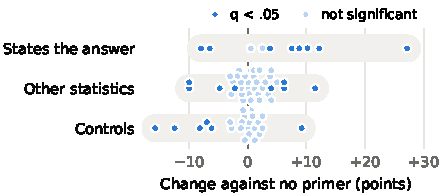
\includegraphics[width=\columnwidth]{fig_effects.pdf}
\caption{Every unflagged cell of Table~\ref{tab:matrix}, one dot per arm, task and primer, grouped by what the primer states. \emph{States the answer}: degree and all three statistics on node degree and edge count; \emph{Controls}: components and filler. Filled: $q<.05$ against no primer.} % [main]
\label{fig:effects}
\end{figure}

\subsection{Stated answers are read off}
\label{sec:readoff}
The degree primer raises node-degree accuracy for plain and thinking 1.7B by $7.5$ and $8.8$ points and lowers it by $6.5$ for plain 4B, which already counts correctly. % [main]
Its gains are largest at intermediate unaided accuracy; at high unaided accuracy it can be a loss (Appendix Figure~\ref{fig:headroom}). % [bands]
On a log-odds scale, which does not compress near ceiling, the loss is plain 4B's alone: at matched unaided accuracy, stated answers break more of its answers than they fix and fix more of plain 1.7B's than they break. % [bandlor]
The same pattern holds within one model. The degree primer hurts plain 4B on the lowest-degree queried nodes in each graph and helps on the highest-degree ones, which have the most neighbors to count ($-11.8$ and $+10.6$ points). % [pdnode]

Reading a value off is itself fallible. Across all seven densities, where the answer is stated, plain 1.7B gets it right less than half the time ($43\%$). Plain 4B stops listing the node's neighbors and reads the value off in most responses at $p=.50$ ($62\%$). A third of its wrong look-ups copy the degree printed one sentence away, more often than chance predicts (Appendix~\ref{app:detail}). % [recover] [route] [copyerr]
The degree primer's effect runs through this change of procedure: plain 4B's loss comes almost wholly from graphs on which its route changed, and thinking 1.7B's gain from graphs on which it did not (\S\ref{sec:thinkmode}). % [routesplit]

\subsection{Side effects include gains and harms}
\label{sec:side}
Filler alone changes up to a fifth of the outcomes in an arm, often on questions primers also change. Identical-prompt rerun flips account for only a minority of each condition's changes (Appendix~\ref{app:detail}).

Side effects differ in sign. On plain 4B edge existence, clustering raises balanced accuracy and RWSE lowers it ($+3.0$ and $-6.5$ points); all three together raise plain 1.7B's but lower plain 4B's (all $q<.05$; Appendix Table~\ref{tab:ee}). % [eemain]
RWSE and all each cost plain 4B $10.0$ points on edge existence. On its dense degree queries, degree alone gains $9.3$, but all loses $21.3$ on the same graphs (Appendix~\ref{app:detail}). % [main] [clusthi]
The largest unflagged gain in Table~\ref{tab:matrix} from a primer without degrees, $+9.2$ on plain 4B neighbor sets, comes from the component sentence. All sampled graphs from $p=.20$ are connected, so the sentence is identical across them. With it the model almost always restates the queried node's line, against about two thirds of responses with no primer and a fifth with filler ($98.5\%$, $63.0\%$, $21.8\%$). Filler moves restatement the other way and costs the same cell $12.5$ points. % [main] [comp] [compproc]

The one side effect that replicates, clustering on plain 1.7B's node degree, is small, specific to that model and to low density, and shows little sign of using the stated values (Appendix~\ref{app:pilot}).

\begin{table}[t]
\centering\scriptsize
\setlength{\tabcolsep}{1.9pt}
\begin{tabular}{llrrrlrr}
\toprule
 & & \multicolumn{2}{c}{\% correct} & \multicolumn{4}{c}{Gap to thinking (points)}\\
\cmidrule(lr){3-4}\cmidrule(lr){5-8}
Task & Model & Plain & Think. & None & \multicolumn{2}{c}{Best primer} & Cl./RW.\\
\midrule
Degree & 1.7B & 60.50 & 76.25 & $\mathbf{+15.8}$ & all & $\mathbf{+5.5}$ & $\mathbf{+11.8}$\\ % [vsthink]
 & 4B & 99.25 & 97.00 & $-2.2$ & components & $\mathbf{-2.5}$ & $-1.8$\\ % [vsthink]
\addlinespace[2pt]
Neighbors & 1.7B & 72.50 & 78.75 & $\mathbf{+6.2}$ & degree & $+2.8$ & $\mathbf{+5.0}$\\ % [vsthink]
 & 4B & 86.00 & 95.50 & $\mathbf{+9.5}$ & components & $+0.2$ & $\mathbf{+8.5}$\\ % [vsthink]
\addlinespace[2pt]
Edge count & 1.7B & 1.25 & 15.75$^{\dagger}$ & $\mathbf{+14.5}$ & degree & $\mathbf{+11.5}$ & $\mathbf{+15.0}$\\ % [vsthink]
 & 4B & 2.00 & 20.00$^{\dagger}$ & $\mathbf{+18.0}$ & degree & $\mathbf{-9.2}$ & $\mathbf{+19.2}$\\ % [vsthink]
\addlinespace[2pt]
Edge exists & 1.7B & 70.50 & 99.00 & $\mathbf{+28.5}$ & all & $\mathbf{+17.0}$ & $\mathbf{+23.5}$\\ % [vsthink]
 & 4B & 90.50 & 99.75 & $\mathbf{+9.2}$ & clustering & $\mathbf{+5.2}$ & $\mathbf{+5.2}$\\ % [vsthink]
\bottomrule
\end{tabular}
\caption{Can a primer close the plain mode's gap to the same model thinking without a primer? \emph{Plain}, \emph{Think.}: correct share without a primer ($p\leq.50$, same graphs). \emph{Gap}: thinking minus plain, in points, first with no primer (\emph{None}), then under the plain model's best primer and under the better of clustering and RWSE (\emph{Cl./RW.}). A gap near $0$ is closed; a negative gap puts the plain mode ahead. Bold: $q<.05$. Chosen on held-out graphs, the best primer is the same in every row. $\dagger$: thinking truncates on most prompts (Table~\ref{tab:truncmatrix}).} % [vsthink] [vscross]
\label{tab:vsthink}
\end{table}

\subsection{Primers against the thinking mode}
\label{sec:vsthink}
Where thinking leads (Table~\ref{tab:vsthink}), the component sentence brings plain 4B's neighbor-set exact match within the $\pm3$-point equivalence margin, on a cell that filler also moves (\S\ref{sec:side}). Elsewhere primers narrow the gap without closing it. All three statistics cut plain 1.7B's node-degree gap to about a third ($15.8$ to $5.5$ points). Under the degree primer its neighbor sets are not significantly below thinking, but the equivalence interval extends beyond the margin. % [vsthink]
Clustering and RWSE close less, and leave the plain mode significantly below thinking wherever thinking leads. The degree primer lifts plain 4B's edge count above thinking. Thinking there is right on nearly every answer it finishes ($97.6\%$), though, so this compares budgets, not ability, and the stated degrees already give the edge count. % [edgecount]

\subsection{Primers in the thinking mode}
\label{sec:thinkmode}
Near ceiling, thinking 4B moves by at most $2.5$ points under any primer on node degree, edge existence and neighbor sets. % [null4bt]
Thinking 1.7B gains from stated degrees (Table~\ref{tab:matrix}) but checks them against its own count instead of reading them off. It keeps listing neighbors, and when its count conflicts with the stated value, it ends on the stated value in two thirds of cases. Checking costs budget: across all seven densities, its node-degree responses that run out of tokens rise from $1.1\%$ to $7.6\%$ under the degree primer. % [trunc]
Where the budget binds, much of any primer's effect is on finishing. Most of thinking 4B's changed answers involve a response that ran out of tokens, and on its edge count even filler gains by lowering truncation (Table~\ref{tab:truncmatrix}).

\subsection{What correct answers rest on}
\label{sec:reston}
Does a primer improve reading the graph itself? By the joint share (\S\ref{sec:method}), clustering and RWSE never do significantly; the degree primer lowers plain 4B's by $9.2$ points and the component sentence raises it by the same amount (Appendix~\ref{app:detail}). % [joint]

Cycle check has the same ``yes'' answer on every sampled graph, but a response can justify it by a real cycle or by the edge count. Without a primer, valid arguments back $34.2\%$ and $58.5\%$ of all prompts for the plain models, and most prompts with thinking. % [ccvalid]
Plain 1.7B rests $43.5\%$ of its correct answers on an invented cycle, one with a step that is not an edge (example in Appendix~\ref{app:detail}). % [ccanswer]
The degree primer raises its valid share to $50.2\%$ yet lowers its accuracy by $17.5$ points. The plain models switch to arguing from the number of edges (Table~\ref{tab:cycles}), a valid route that, like a look-up, need not read the edges. RWSE, all three statistics and filler lower plain 4B's valid share. % [ccvalid] [main]

\section{Discussion}
\label{sec:discussion}
A stated degree is worth what counting it from the incident list costs (\S\ref{sec:readoff}), and a look-up is not free either: it must match the right node to the right sentence, and wrong look-ups show where that fails.

Some structural encodings help message-passing GNNs by supplying what they cannot compute: return probabilities separate nodes that 1-WL-bounded networks cannot \citep{xu2019powerful,dwivedi2022graph}. A language model has the information instead: every edge is in its context, and thinking 4B answers nearly all degree, neighbor-set and edge-existence queries (Table~\ref{tab:vsthink}). The gap to thinking suggests that the plain models' bottleneck is computation, not information, so a statistic can help by stating the answer or by changing how the text is read. Clustering and RWSE state no answer: their text reveals degrees mainly in sparse graphs (\S\ref{sec:states}) and almost nothing about edge existence (Table~\ref{tab:solver}). Their effects, which vary in sign, mostly reflect how the text is read.

Raw accuracy can also mislead: on dense graphs plain 1.7B's edge-existence accuracy rises steeply while its balanced accuracy stays near chance. % [fillerdens] [collapse]

\section{Future Work}
\label{sec:future}
First, corrupt or omit the queried node's stated degree, keeping all else fixed, to separate following a stated value, checking it and counting from edges. Second, shuffle node labels and primer order, and test the component sentence against neutral text of equal length and position; the same controls apply to clustering's low-density degree gain. Third, sample acyclic as well as cyclic graphs, and families that vary triangles at matched size and density, so that cycle check has two answers and clustering carries information. Other model families, larger thinking budgets and a graph-counting tool would show when a primer is the cheapest way to supply a computation.

\section{Conclusion}
\label{sec:conclusion}
We asked three questions. \emph{Does a structural primer help?} Mainly by stating the answer: a stated degree saves an unreliable count and disturbs a reliable one, and adding clustering and RWSE need not preserve its effect. \emph{Does matching the statistic to the task matter?} Yes: clustering and RWSE, which state no answer, have mostly small effects of either sign and never significantly improve execution; plain Qwen3-1.7B's rises by about $4$ points under both, below what we can detect; the component sentence changes plain Qwen3-4B's procedure instead. \emph{Does capacity matter?} Through unaided accuracy: stated degrees help Qwen3-1.7B and hurt plain Qwen3-4B, yet also help plain Qwen3-4B on dense graphs, where its own count fails (Appendix~\ref{app:detail}). Thinking mostly keeps its lead. Beside paired controls, completion rates and graph-checked claims show whether an answer was supplied, the incident line read, or a correct label validly argued. % [joint]

\section*{Limitations}
\emph{Scope:} two Qwen3 models (and Qwen3-8B in one follow-up); independent-edge graphs of $40$ nodes ($20$--$160$ in one follow-up); one encoding, one wording and position per primer; zero-shot; fixed token budgets. \emph{Controls:} filler matches only clustering's length; component count is structural information; no primer has shuffled or wrong values, and no instruction-only baseline isolates procedural wording. Nodes 0--9, listed first, also have the shortest ids, so position and id length are confounded. \emph{Measurement:} response readers other than conflict detection were spot-checked by an LLM, not blind hand labels.

\clearpage
\bibliography{custom}
\bibliographystyle{acl_natbib}
\clearpage
\appendix
% Appendix floats: float-only columns and pages stack from the top, and sit closer to the text.
\makeatletter
\setlength{\@fptop}{0pt}\setlength{\@fpsep}{\floatsep}
\setlength{\@dblfptop}{0pt}\setlength{\@dblfpsep}{\dblfloatsep}
\makeatother
\setlength{\textfloatsep}{10pt plus 2pt minus 2pt}
\setlength{\dbltextfloatsep}{10pt plus 2pt minus 2pt}
\setlength{\intextsep}{8pt plus 2pt minus 2pt}
\renewcommand{\topfraction}{0.9}\renewcommand{\dbltopfraction}{0.9}\renewcommand{\textfraction}{0.1}\setcounter{topnumber}{3}\setcounter{dbltopnumber}{2}
\section{Method Details}
\label{app:audit}

\paragraph{Statistics.} With adjacency matrix $A$ and transition matrix $P=D^{-1}A$, the per-node statistics are $d_v=\sum_u A_{vu}$, $c_v=2t_v/(d_v(d_v-1))$ and $r_v^{(k)}=(P^k)_{vv}$ for $k\in\{2,3\}$, where $t_v$ counts edges among $v$'s neighbors and $c_v=0$ when $d_v<2$. Clustering and return probabilities are printed to two decimals, one sentence per node, in node order (Table~\ref{tab:primerlength}).

\paragraph{Why these features.} Degree and RWSE are the structural encodings graph Transformers use \citep{rampasek2022recipe}. Local clustering adds how a node's neighbors connect. The component count is a single global fact that, with the node and edge counts, decides whether a cycle exists. Laplacian encodings are excluded because eigenvector signs and bases need an explicit convention \citep{dwivedi2022graph}. RWSE keeps only $k=2,3$: $r_v^{(1)}=0$ in every simple graph, $k=3$ detects triangles, and within a graph degree and clustering already explain most of the variance of $k=4$ and $k=5$.

\paragraph{Models, budgets and power.} Models are the Qwen3 checkpoints on Hugging Face, run with \texttt{transformers}. Each response may use up to $8{,}192$ new tokens, and $2{,}048$ for the plain arms at $p\geq.65$, where no arm truncates more than $2.5\%$ of its responses. The main sweep and its extension hold $84{,}000$ responses on $700$ graphs. % [setup] [extract]
In one $100$-graph cell the median smallest detectable paired effect is $7.4$ points, and $13.7$ where side information meets intermediate accuracy. % [power]
Under one BH correction over all $264$ tests, every bold cell of Table~\ref{tab:matrix} but one and all but three $^{\mathrm{f}}$ marks stay significant. % [globalbh]
Greedy generation is not exactly reproducible: generating the same prompts twice changes the outcome of $5.3\%$, so we compare net paired changes, never counts of changed answers. % [rerun]

\paragraph{Graph-blind solver.} It reads only the primer text, with $16$ exact rules, $1$ heuristic and $8$ rules fitted on graphs disjoint from those scored (Table~\ref{tab:solver}). % [bars] [leak]

\begin{table}[h]
\centering\scriptsize
\setlength{\tabcolsep}{4pt}
\begin{tabular}{lrrrr}
\toprule
Primer & Degree & Neighbors & Edge count & Edge exists\\
\midrule
none & 14.4 & 0.0 & 3.0 & 73.5\\ % [bars]
degree & 100.0 & 0.1 & 100.0 & 74.6\\ % [bars]
clustering & 14.4 & 0.0 & 10.4 & 72.7\\ % [bars]
RWSE & 21.0 & 0.1 & 3.0 & 55.4\\ % [bars]
all & 100.0 & 0.8 & 100.0 & 74.1\\ % [bars]
components & 14.4 & 0.0 & 3.0 & 73.5\\ % [bars]
filler & 14.4 & 0.0 & 3.0 & 73.5\\ % [bars]
\bottomrule
\end{tabular}
\caption{Graph-blind solver accuracy (\%) from the primer text alone, 40-node graphs, averaged over all seven densities ($p=.10$--$.85$), on the four tasks whose answer varies. RWSE falls below no primer on edge existence because a fitted density threshold fails at $p\geq.65$ ($38.0$, $48.0$ and $12.0\%$).} % [bars] [blindbar]
\label{tab:solver}
\end{table}

\begin{table}[h]
\centering\footnotesize
\setlength{\tabcolsep}{4pt}
\begin{tabular}{lrp{3.1cm}}
\toprule
Primer & Mean chars & Information\\
\midrule
degree & 891 & Degree for each node\\ % [length]
clustering & 1,629 & Local clustering for each node\\ % [length]
RWSE & 2,949 & Two rounded return values per node\\ % [length]
all & 4,691 & Degree, clustering and RWSE\\ % [length]
components & 37 & Number of connected components\\ % [length]
filler & 1,829 & Node names, no graph statistic\\ % [length]
\bottomrule
\end{tabular}
\caption{Mean preamble length in characters over the main-sweep graphs.} % [length]
\label{tab:primerlength}
\end{table}

\paragraph{Response readers.} A response is a look-up when it answers without restating the queried node's neighbor list, and lists the neighbors when it gives five or more one per line. The cycle and edge readers check every asserted step against the prompt's graph.
\paragraph{Scoring.} The answer extractor parses $99.84\%$ of responses. Set-F1 on neighbor sets is secondary because it gives partial credit: it moves in the same direction as exact match in $3$ of $5$ large contrasts, and by $0.11$ to $0.17$ as much. Balanced-accuracy changes use a paired permutation test with Benjamini--Hochberg adjustment over the six conditions within an arm. % [extract] [f1] [eemain]Under one BH correction over all $264$ tests, the bold cell of Table~\ref{tab:matrix} that loses significance has $q=.057$, and the three $^{\mathrm{f}}$ marks $q=.055$--$.088$. % [globalbh]

\section{Detailed Results}
\label{app:detail}
\label{app:more}
\label{app:tables}
Tables~\ref{tab:full} and~\ref{tab:truncmatrix} complete Table~\ref{tab:matrix} with $95\%$ intervals, truncated shares and the two constant-answer tasks. The paragraphs below give the numbers Section~\ref{sec:results} summarizes, in its order.

\begin{table*}[t]
\centering\scriptsize
\setlength{\tabcolsep}{2pt}
\resizebox{\textwidth}{!}{%
\begin{tabular}{llrrrrrr}
\toprule
Task & Arm & degree & clustering & RWSE & all & components & filler\\
\midrule
Degree & 1.7P & $+7.5$ {\tiny$[+3.0,+11.8]$} & $+3.0$ {\tiny$[-1.5,+7.5]$} & $+4.0$ {\tiny$[-0.5,+8.5]$} & $+10.2$ {\tiny$[+5.2,+15.2]$} & $+1.8$ {\tiny$[-2.2,+5.8]$} & $-0.5$ {\tiny$[-4.2,+3.5]$}\\ % [main]
 & 1.7T & $+8.8$ {\tiny$[+4.2,+13.2]$} & $+1.5$ {\tiny$[-2.5,+5.5]$} & $+2.5$ {\tiny$[-2.0,+6.8]$} & $+12.2$ {\tiny$[+8.0,+16.5]$} & $-1.0$ {\tiny$[-4.2,+2.5]$} & $-3.0$ {\tiny$[-7.0,+0.8]$}\\ % [main]
 & 4P & $-6.5$ {\tiny$[-9.2,-4.0]$} & $-0.5$ {\tiny$[-2.0,+0.8]$} & $-2.2$ {\tiny$[-4.2,-0.5]$} & $-8.0$ {\tiny$[-11.0,-5.2]$} & $+0.2$ {\tiny$[+0.0,+0.8]$} & $-0.5$ {\tiny$[-2.0,+1.0]$}\\ % [main]
 & 4T & $+2.5$ {\tiny$[+0.8,+4.2]$} & $+1.8$ {\tiny$[-0.2,+3.8]$} & $-1.2$ {\tiny$[-3.8,+1.0]$} & $+0.5$ {\tiny$[-1.5,+2.8]$} & $+0.2$ {\tiny$[-1.8,+2.5]$} & $+2.0$ {\tiny$[+0.5,+3.8]$}\\ % [main]
\addlinespace[1pt]
Neighbors & 1.7P & $+3.5$ {\tiny$[-0.5,+7.2]$} & $+1.2$ {\tiny$[-3.0,+5.5]$} & $+1.0$ {\tiny$[-3.2,+5.2]$} & $+2.0$ {\tiny$[-2.5,+6.5]$} & $+0.8$ {\tiny$[-2.5,+4.5]$} & $-6.2$ {\tiny$[-10.5,-2.2]$}\\ % [main]
 & 1.7T & $+6.2$ {\tiny$[+2.8,+10.0]$} & $+2.0$ {\tiny$[-2.0,+6.0]$} & $+0.2$ {\tiny$[-3.5,+4.0]$} & $+6.2$ {\tiny$[+2.5,+10.0]$} & $+2.5$ {\tiny$[-0.8,+6.0]$} & $+2.5$ {\tiny$[-1.0,+6.0]$}\\ % [main]
 & 4P & $-3.0$ {\tiny$[-7.0,+1.0]$} & $+1.0$ {\tiny$[-2.8,+4.8]$} & $+0.0$ {\tiny$[-3.8,+4.0]$} & $-2.8$ {\tiny$[-7.0,+1.8]$} & $+9.2$ {\tiny$[+6.0,+12.8]$} & $-12.5$ {\tiny$[-17.2,-7.8]$}\\ % [main]
 & 4T & $+0.5$ {\tiny$[-2.2,+3.2]$} & $-0.8$ {\tiny$[-3.2,+1.8]$} & $+0.5$ {\tiny$[-1.8,+3.0]$} & $-1.2$ {\tiny$[-3.8,+1.2]$} & $+0.5$ {\tiny$[-1.8,+2.8]$} & $+1.2$ {\tiny$[-1.0,+3.5]$}\\ % [main]
\addlinespace[1pt]
Edge count & 1.7P & $+3.0$$^\dagger$ {\tiny$[+0.8,+5.2]$} & $-0.5$$^\dagger$ {\tiny$[-2.0,+1.0]$} & $-0.8$$^\dagger$ {\tiny$[-2.0,+0.5]$} & $+0.8$$^\dagger$ {\tiny$[-1.0,+2.5]$} & $-1.0$$^\dagger$ {\tiny$[-2.2,+0.0]$} & $-0.5$$^\dagger$ {\tiny$[-1.8,+0.8]$}\\ % [main]
 & 1.7T & $-3.2$$^\dagger$ {\tiny$[-7.8,+1.2]$} & $-1.2$$^\dagger$ {\tiny$[-5.5,+3.0]$} & $-3.2$$^\dagger$ {\tiny$[-7.2,+0.5]$} & $+5.0$$^\dagger$ {\tiny$[+0.2,+10.0]$} & $-0.8$$^\dagger$ {\tiny$[-5.0,+3.8]$} & $-1.5$$^\dagger$ {\tiny$[-5.5,+2.5]$}\\ % [main]
 & 4P & $+27.2$ {\tiny$[+22.8,+32.0]$} & $-1.2$ {\tiny$[-3.0,+0.2]$} & $-1.5$ {\tiny$[-3.0,-0.2]$} & $+3.8$ {\tiny$[+1.2,+6.2]$} & $-1.2$ {\tiny$[-2.8,+0.0]$} & $+1.2$ {\tiny$[-0.8,+3.0]$}\\ % [main]
 & 4T & $+8.5$$^\dagger$ {\tiny$[+3.2,+14.2]$} & $+24.8$$^\dagger$ {\tiny$[+19.5,+30.2]$} & $+10.2$$^\dagger$ {\tiny$[+5.5,+15.0]$} & $+1.8$$^\dagger$ {\tiny$[-3.5,+7.2]$} & $+24.8$$^\dagger$ {\tiny$[+19.8,+30.0]$} & $+12.2$$^\dagger$ {\tiny$[+7.2,+17.0]$}\\ % [main]
\addlinespace[1pt]
Edge exists & 1.7P & $+4.0$ {\tiny$[-0.2,+8.2]$} & $+3.8$ {\tiny$[-0.5,+8.0]$} & $+5.0$ {\tiny$[+0.2,+9.5]$} & $+11.5$ {\tiny$[+6.2,+16.5]$} & $-8.2$ {\tiny$[-11.8,-4.8]$} & $-15.8$ {\tiny$[-20.0,-11.8]$}\\ % [main]
 & 1.7T & $-2.5$ {\tiny$[-4.5,-0.8]$} & $-1.0$ {\tiny$[-2.8,+0.5]$} & $-1.2$ {\tiny$[-3.0,+0.5]$} & $-1.8$ {\tiny$[-3.8,+0.0]$} & $-0.8$ {\tiny$[-2.5,+0.8]$} & $-0.5$ {\tiny$[-2.0,+1.0]$}\\ % [main]
 & 4P & $-4.8$ {\tiny$[-7.8,-1.5]$} & $+4.0$ {\tiny$[+1.0,+7.0]$} & $-10.0$ {\tiny$[-13.8,-6.2]$} & $-10.0$ {\tiny$[-14.0,-6.0]$} & $-2.8$ {\tiny$[-5.8,+0.2]$} & $-7.0$ {\tiny$[-10.5,-3.5]$}\\ % [main]
 & 4T & $+0.0$ {\tiny$[-0.8,+0.8]$} & $-0.8$ {\tiny$[-1.8,+0.0]$} & $-1.2$ {\tiny$[-2.5,+0.0]$} & $-1.0$ {\tiny$[-2.2,+0.0]$} & $-0.5$ {\tiny$[-1.5,+0.5]$} & $+0.0$ {\tiny$[+0.0,+0.0]$}\\ % [main]
\addlinespace[1pt]
Node count & 1.7P & $+6.8$ {\tiny$[+3.2,+10.5]$} & $+67.2$ {\tiny$[+64.5,+70.0]$} & $+2.0$ {\tiny$[-3.2,+6.8]$} & $+47.0$ {\tiny$[+42.5,+51.2]$} & $+21.2$ {\tiny$[+16.2,+26.2]$} & $+39.8$ {\tiny$[+36.0,+43.5]$}\\ % [main]
 & 1.7T & $+5.5$ {\tiny$[+2.5,+8.5]$} & $+9.0$ {\tiny$[+6.5,+11.8]$} & $+9.0$ {\tiny$[+6.5,+11.8]$} & $+9.0$ {\tiny$[+6.5,+11.8]$} & $+1.5$ {\tiny$[-2.2,+5.0]$} & $+9.0$ {\tiny$[+6.5,+11.8]$}\\ % [main]
 & 4P & $+8.0$ {\tiny$[+5.2,+10.8]$} & $+8.8$ {\tiny$[+6.0,+11.5]$} & $+9.2$ {\tiny$[+6.5,+12.0]$} & $+9.8$ {\tiny$[+7.2,+12.5]$} & $+9.0$ {\tiny$[+6.5,+11.8]$} & $+9.2$ {\tiny$[+6.8,+11.8]$}\\ % [main]
 & 4T & $+0.2$ {\tiny$[-0.5,+1.2]$} & $+0.2$ {\tiny$[-0.5,+1.2]$} & $+0.2$ {\tiny$[-0.5,+1.2]$} & $+0.5$ {\tiny$[+0.0,+1.2]$} & $+0.0$ {\tiny$[-1.0,+1.0]$} & $+0.5$ {\tiny$[+0.0,+1.2]$}\\ % [main]
\addlinespace[1pt]
Cycle & 1.7P & $-17.5$$^\dagger$ {\tiny$[-23.0,-12.2]$} & $+8.5$ {\tiny$[+5.8,+11.2]$} & $-0.2$ {\tiny$[-4.2,+3.5]$} & $+7.0$ {\tiny$[+4.0,+10.2]$} & $+2.0$ {\tiny$[-1.5,+5.3]$} & $+3.0$ {\tiny$[-0.8,+6.8]$}\\ % [main]
 & 1.7T & $-21.8$$^\dagger$ {\tiny$[-26.5,-17.5]$} & $-0.5$ {\tiny$[-2.8,+1.8]$} & $+2.2$ {\tiny$[+0.5,+4.0]$} & $-0.8$ {\tiny$[-3.2,+1.8]$} & $-7.5$ {\tiny$[-11.0,-4.2]$} & $+3.0$ {\tiny$[+1.5,+4.8]$}\\ % [main]
 & 4P & $-2.2$ {\tiny$[-4.2,-0.5]$} & $+0.5$ {\tiny$[-0.5,+1.8]$} & $-0.2$ {\tiny$[-1.8,+1.2]$} & $-0.2$ {\tiny$[-1.8,+1.0]$} & $-2.0$ {\tiny$[-4.0,-0.2]$} & $-0.5$ {\tiny$[-2.0,+0.8]$}\\ % [main]
 & 4T & $-5.5$ {\tiny$[-8.0,-3.0]$} & $+0.0$ {\tiny$[-1.2,+1.2]$} & $+0.2$ {\tiny$[-0.8,+1.5]$} & $-0.5$ {\tiny$[-2.0,+0.8]$} & $-3.2$ {\tiny$[-5.2,-1.2]$} & $+0.5$ {\tiny$[-0.5,+1.5]$}\\ % [main]
\bottomrule
\end{tabular}}
\caption{Every main-sweep effect against no primer (points) with its $95\%$ bootstrap interval over graphs, $400$ paired graphs per cell ($p\leq.50$). $\dagger$: at least $15\%$ truncation on either side. Node count (always $40$) and cycle check (always yes) cannot measure reading the graph at $40$ nodes. P/T: plain/thinking.} % [main]
\label{tab:full}
\end{table*}

\begin{figure}[!h]
\centering
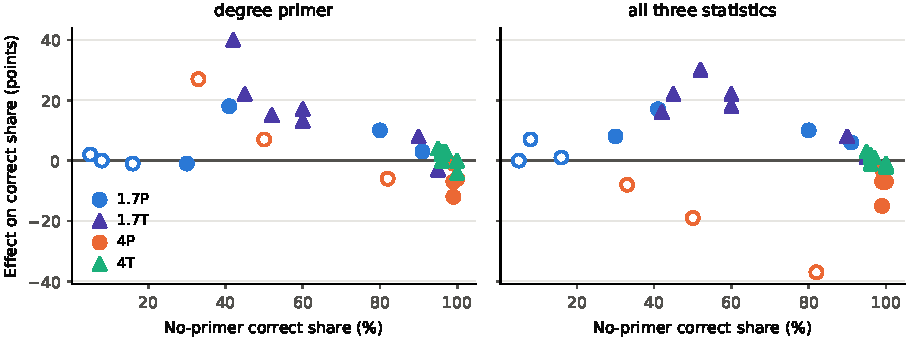
\includegraphics[width=\columnwidth]{fig_headroom.pdf}
\caption{The degree primer's effect on node degree against the no-primer correct share, per arm and density. Hollow: plain arm at $p\geq.65$ (smaller budget).} % [flip] [bands]
\label{fig:headroom}
\end{figure}

\paragraph{Stated answers (\S\ref{sec:readoff}).} The gain follows the room the model leaves (Figure~\ref{fig:headroom}). In node-degree cells answered $25$--$50\%$ and $50$--$75\%$ correctly without them, answer-stating primers gain $16.1$ and $12.9$ points; at $75$--$90\%$ they lose $5.8$. These bands hold on held-out halves of the graphs and with the truncation flag at $10\%$ or $50\%$ (at least $+12.5$ in every case). % [bands] [splithalf] [bandsens]
An effect mostly follows how well the model does unaided. At a fixed accuracy without a primer, density adds little ($p=.28$ for answer-stating primers, $p=.85$ for side statistics), except that side statistics' effect on node degree falls with density ($p=.006$). % [dxbase]
One model falls on both sides. The degree primer costs plain 4B $12.0$ points at $p=.50$, where it answers $99.0\%$ correctly unaided, and gains $27.0$ at $p=.85$, where it answers $33.0\%$ (both $q<.01$). % [flip]
Stated answers are not always taken: across all seven densities, where the solver scores $100\%$, node-degree accuracy under the degree primer is $43\%$ and $81\%$ for plain 1.7B and plain 4B, and $79\%$ and $98\%$ with thinking. At high density, where plain 1.7B is weakest, the stated degree barely helps it (at most $2$ points). At $p=.85$ it still answers $39$, the degree of a node joined to all others, on $70.8\%$ of finished responses. % [recover] [plain17] [ddplain]
Plain 4B's wrong look-ups copy a nearby line: $17$ of $57$ equal the degree printed one sentence away, against $10.4$ expected by chance ($p=.017$). Adding clustering and RWSE to the same degrees costs dense plain 4B the most (Figure~\ref{fig:addstats}): pooled over $p\geq.65$, degree alone gains $9.3$ points ($q=.03$) and all three statistics lose $21.3$ ($q<.001$). % [copyerr] [clusthi]
\begin{figure}[!h]
\centering
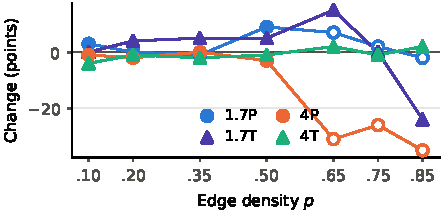
\includegraphics[width=\columnwidth]{fig_addstats.pdf}
\caption{What adding clustering and RWSE to the same degrees changes on node degree (all three statistics minus the degree primer, points), per arm and density. Hollow as in Figure~\ref{fig:headroom}.}
\label{fig:addstats}
\end{figure}

\paragraph{Filler and fragile questions (\S\ref{sec:side}).} Filler changes $6.2$--$18.6\%$ of outcomes per arm. % [churn]
A primer changes $38.5$--$69.1\%$ of the questions filler changes and $3.1$--$15.2\%$ of the rest. % [overlap]
Some questions are fragile: on plain 1.7B's node degree, $24$ of $400$ change outcome when the same prompt is generated again. Every condition changes them far more often than the rest ($45.8$--$66.7\%$ against $14.4$--$26.1\%$, $q\leq.018$). Yet they carry only $11$ to $16$ of each condition's $65$ to $113$ changes, a lower bound on chance with only two generations per prompt. % [rerunflip]
Where accuracy without a primer is $25$--$75\%$, components, clustering and RWSE average $+1.6$ points while filler averages $-6.9$ on the same cells. % [fillerband]

\begin{table}[!t]
\centering\footnotesize\setlength{\tabcolsep}{4pt}
\begin{tabular}{llrrr}
\toprule
Arm & Primer & Raw & Balanced & Yes\\
\midrule
1.7P & none & 70.50 & 79.86 & 56.2\\ % [eemain] (%)
 & degree & 74.50 & 82.30 & 51.7\\ % [eemain] (%)
 & clustering & 74.25 & 82.42 & 52.5\\ % [eemain] (%)
 & RWSE & 75.50 & 82.68 & 50.1\\ % [eemain] (%)
 & all & 82.00 & \textbf{87.71} & 44.8\\ % [eemain] (%)
 & components & 62.25 & \textbf{74.23} & 64.5\\ % [eemain] (%)
 & filler & 54.75 & \textbf{69.11} & 72.0\\ % [eemain] (%)
\addlinespace[2pt]
1.7T & none & 99.00 & 99.02 & 27.1\\ % [eemain] (%)
 & degree & 96.50 & 97.61 & 29.9\\ % [eemain] (%)
 & clustering & 98.00 & 98.63 & 28.6\\ % [eemain] (%)
 & RWSE & 97.75 & 98.17 & 28.3\\ % [eemain] (%)
 & all & 97.25 & 98.12 & 29.5\\ % [eemain] (%)
 & components & 98.25 & 98.81 & 28.3\\ % [eemain] (%)
 & filler & 98.50 & 98.68 & 27.8\\ % [eemain] (%)
\addlinespace[2pt]
4P & none & 90.50 & 93.22 & 35.7\\ % [eemain] (%)
 & degree & 85.75 & \textbf{90.27} & 40.7\\ % [eemain] (%)
 & clustering & 94.50 & \textbf{96.25} & 32.3\\ % [eemain] (%)
 & RWSE & 80.50 & \textbf{86.69} & 46.3\\ % [eemain] (%)
 & all & 80.50 & \textbf{86.69} & 46.1\\ % [eemain] (%)
 & components & 87.75 & 91.64 & 39.0\\ % [eemain] (%)
 & filler & 83.50 & \textbf{88.74} & 43.2\\ % [eemain] (%)
\addlinespace[2pt]
4T & none & 99.75 & 99.83 & 26.8\\ % [eemain] (%)
 & degree & 99.75 & 99.83 & 26.8\\ % [eemain] (%)
 & clustering & 99.00 & 99.32 & 27.0\\ % [eemain] (%)
 & RWSE & 98.50 & 98.68 & 26.9\\ % [eemain] (%)
 & all & 98.75 & 99.15 & 27.1\\ % [eemain] (%)
 & components & 99.25 & 99.49 & 27.0\\ % [eemain] (%)
 & filler & 99.75 & 99.83 & 26.8\\ % [eemain] (%)
\bottomrule
\end{tabular}
\caption{Edge existence, main sweep ($400$ prompts per row): raw and balanced accuracy over all prompts and the share of finished answers that say yes, all in \%. Truncation is in Table~\ref{tab:truncmatrix}. Bold: balanced accuracy differs from the same arm without a primer (paired permutation, BH $q<.05$ within arm).} % [eemain]
\label{tab:ee}
\end{table}

\begin{table}[!t]
\centering\scriptsize
\setlength{\tabcolsep}{3.4pt}
\begin{tabular}{@{}llrrrrrr@{}}
\toprule
 & & Correct & \multicolumn{3}{c}{Cycle named} & \multicolumn{2}{c}{No cycle}\\
\cmidrule(lr){4-6}\cmidrule(l){7-8}
Arm & Primer & ``yes'' & Real & Invented & Not a & Total & Edge\\
 & & ($n$) & & & cycle & & count\\
\midrule
1.7P & none & 363 & 36.9 & 43.5 & 16.0 & 3.6 & 0.8\\ % [ccanswer] [cctest]
 & degree & 293 & \textbf{13.0} & \textbf{20.5} & 1.4 & 65.2 & 55.6\\ % [ccanswer] [cctest]
 & clustering & 397 & 39.5 & 48.1 & 7.8 & 4.5 & 1.0\\ % [ccanswer] [cctest]
 & RWSE & 362 & 33.7 & 40.3 & 19.9 & 6.1 & 1.7\\ % [ccanswer] [cctest]
 & all & 391 & 38.4 & 50.4 & 7.9 & 3.3 & 1.3\\ % [ccanswer] [cctest]
 & components & 371 & \textbf{27.8} & 40.4 & 25.3 & 6.5 & 4.3\\ % [ccanswer] [cctest]
 & filler & 375 & 33.3 & \textbf{55.5} & 9.6 & 1.6 & 0.0\\ % [ccanswer] [cctest]
\addlinespace[2pt]
1.7T & none & 388 & 79.9 & 17.8 & 1.0 & 1.3 & 0.5\\ % [ccanswer] [cctest]
 & degree & 301 & \textbf{61.5} & \textbf{29.6} & 0.0 & 9.0 & 9.0\\ % [ccanswer] [cctest]
 & clustering & 386 & 80.6 & 19.2 & 0.0 & 0.3 & 0.3\\ % [ccanswer] [cctest]
 & RWSE & 397 & \textbf{68.0} & 20.7 & 10.6 & 0.8 & 0.5\\ % [ccanswer] [cctest]
 & all & 385 & 73.0 & 21.8 & 3.1 & 2.1 & 1.8\\ % [ccanswer] [cctest]
 & components & 358 & 74.9 & 22.6 & 0.0 & 2.5 & 2.0\\ % [ccanswer] [cctest]
 & filler & 400 & 77.2 & 19.8 & 2.5 & 0.5 & 0.0\\ % [ccanswer] [cctest]
\addlinespace[2pt]
4P & none & 396 & 34.1 & 23.0 & 6.8 & 36.1 & 25.0\\ % [ccanswer] [cctest]
 & degree & 387 & \textbf{13.4} & \textbf{3.9} & 2.1 & 80.6 & 65.6\\ % [ccanswer] [cctest]
 & clustering & 398 & \textbf{48.7} & \textbf{31.2} & 1.0 & 19.1 & 5.8\\ % [ccanswer] [cctest]
 & RWSE & 395 & 33.2 & 20.8 & 38.7 & 7.3 & 0.5\\ % [ccanswer] [cctest]
 & all & 395 & \textbf{45.1} & \textbf{33.4} & 6.6 & 14.9 & 0.8\\ % [ccanswer] [cctest]
 & components & 388 & 39.2 & 18.6 & 3.4 & 38.9 & 26.5\\ % [ccanswer] [cctest]
 & filler & 394 & \textbf{44.2} & 28.2 & 5.3 & 22.3 & 2.3\\ % [ccanswer] [cctest]
\addlinespace[2pt]
4T & none & 397 & 96.5 & 3.3 & 0.0 & 0.3 & 0.0\\ % [ccanswer] [cctest]
 & degree & 375 & \textbf{90.9} & 5.1 & 0.0 & 4.0 & 2.7\\ % [ccanswer] [cctest]
 & clustering & 397 & 95.5 & 4.5 & 0.0 & 0.0 & 0.0\\ % [ccanswer] [cctest]
 & RWSE & 398 & \textbf{55.0} & 2.5 & 42.5 & 0.0 & 0.0\\ % [ccanswer] [cctest]
 & all & 395 & 92.7 & 6.3 & 0.0 & 1.0 & 1.0\\ % [ccanswer] [cctest]
 & components & 384 & \textbf{92.2} & 4.4 & 0.0 & 3.4 & 2.9\\ % [ccanswer] [cctest]
 & filler & 399 & 94.2 & 5.0 & 0.5 & 0.3 & 0.0\\ % [ccanswer] [cctest]
\bottomrule
\end{tabular}
\caption{What the correct cycle-check answers rest on (main sweep; every correct answer is ``yes''). \emph{Correct ($n$)}: count of correct, finished answers; the other columns are \% of those $n$, and Real, Invented, Not a cycle and Total sum to 100. \emph{Real}: every step of the cycle is an edge; \emph{Invented}: a step is not an edge; \emph{Not a cycle}: a length-2 or retraced walk. \emph{Edge count}: the answers under Total that argue from the number of edges, identified by their wording. The valid arguments are Real and Edge count, which is valid because $40$ nodes with at least $40$ edges must contain a cycle. Bold (Real, Invented only): differs from the same model without a primer (paired, BH $q<.05$).} % [ccanswer] [cctest]
\label{tab:cycles}
\end{table}


\begin{table*}[t]
\centering\scriptsize
\setlength{\tabcolsep}{3.4pt}
\begin{tabular}{llrrrrrrr}
\toprule
Task & Arm & none & degree & clustering & RWSE & all & components & filler\\
\midrule
Degree & 1.7P & 0.00 & $+0.0$ & $+0.0$ & $+0.2$ & $+0.0$ & $+0.0$ & $+0.0$\\ % [main] [trunc]
 & 1.7T & 0.75 & $+4.5$ & $-0.5$ & $+0.0$ & $-0.5$ & $-0.2$ & $-0.5$\\ % [main] [trunc]
 & 4P & 0.00 & $+0.0$ & $+0.0$ & $+0.0$ & $+0.0$ & $+0.0$ & $+0.0$\\ % [main] [trunc]
 & 4T & 2.75 & $-2.5$ & $-2.0$ & $-0.5$ & $-1.0$ & $-0.5$ & $-1.8$\\ % [main] [trunc]
\addlinespace[2pt]
Neighbors & 1.7P & 0.00 & $+0.0$ & $+0.0$ & $+0.0$ & $+0.2$ & $+0.0$ & $+0.0$\\ % [main] [trunc]
 & 1.7T & 1.25 & $+0.2$ & $-1.0$ & $-0.8$ & $-0.5$ & $-0.2$ & $-0.8$\\ % [main] [trunc]
 & 4P & 0.00 & $+0.0$ & $+0.0$ & $+0.0$ & $+0.0$ & $+0.0$ & $+0.0$\\ % [main] [trunc]
 & 4T & 3.25 & $-0.2$ & $+1.2$ & $-0.2$ & $+1.0$ & $+0.2$ & $-0.5$\\ % [main] [trunc]
\addlinespace[2pt]
Edge count & 1.7P & 29.75 & $-20.2$ & $-11.8$ & $-11.8$ & $-1.8$ & $-2.5$ & $-3.5$\\ % [main] [trunc]
 & 1.7T & 81.75 & $-0.8$ & $+0.8$ & $+5.0$ & $-12.2$ & $+0.5$ & $+1.2$\\ % [main] [trunc]
 & 4P & 0.00 & $+1.8$ & $+0.2$ & $+0.5$ & $+0.8$ & $+0.8$ & $+0.0$\\ % [main] [trunc]
 & 4T & 79.50 & $-20.8$ & $-26.0$ & $-12.2$ & $-23.8$ & $-25.0$ & $-13.0$\\ % [main] [trunc]
\addlinespace[2pt]
Edge exists & 1.7P & 0.00 & $+0.0$ & $+0.0$ & $+0.2$ & $+0.0$ & $+0.0$ & $+0.0$\\ % [main] [trunc]
 & 1.7T & 0.25 & $+0.2$ & $+0.0$ & $+0.0$ & $-0.2$ & $+0.0$ & $-0.2$\\ % [main] [trunc]
 & 4P & 0.00 & $+0.5$ & $+0.0$ & $+0.0$ & $+0.2$ & $+0.0$ & $+0.0$\\ % [main] [trunc]
 & 4T & 0.25 & $+0.0$ & $+0.8$ & $+1.2$ & $+1.0$ & $+0.5$ & $+0.0$\\ % [main] [trunc]
\midrule
Node count & 1.7P & 0.00 & $+0.0$ & $+0.0$ & $+0.0$ & $+0.0$ & $+0.0$ & $+0.0$\\ % [main] [trunc]
 & 1.7T & 7.75 & $-5.0$ & $-7.8$ & $-7.8$ & $-7.8$ & $-0.5$ & $-7.8$\\ % [main] [trunc]
 & 4P & 0.00 & $+0.0$ & $+0.0$ & $+0.0$ & $+0.0$ & $+0.0$ & $+0.0$\\ % [main] [trunc]
 & 4T & 0.00 & $+0.2$ & $+0.2$ & $+0.2$ & $+0.0$ & $+0.0$ & $+0.0$\\ % [main] [trunc]
\addlinespace[2pt]
Cycle & 1.7P & 9.00 & $+8.2$ & $-8.2$ & $-7.2$ & $-8.0$ & $-2.5$ & $-2.8$\\ % [main] [trunc]
 & 1.7T & 3.00 & $+21.2$ & $+0.5$ & $-2.2$ & $+0.8$ & $+7.5$ & $-3.0$\\ % [main] [trunc]
 & 4P & 0.75 & $+0.8$ & $-0.2$ & $+0.5$ & $-0.2$ & $+0.8$ & $+0.5$\\ % [main] [trunc]
 & 4T & 0.75 & $+4.8$ & $+0.0$ & $-0.2$ & $+0.5$ & $+3.2$ & $-0.5$\\ % [main] [trunc]
\bottomrule
\end{tabular}
\caption{Complete main-sweep truncated shares: no-primer baseline (percent of all prompts) and paired changes (percentage points), for the same queries as Table~\ref{tab:full}. Each of its cells' \emph{wrong} share equals $100\%$ minus its correct and truncated shares. P/T: plain/thinking; components and filler are diagnostics. No significance marks are assigned to truncation contrasts.} % [setup] [main]
\label{tab:truncmatrix}
\end{table*}


\paragraph{Side statistics (\S\ref{sec:side}).} On edge existence, every primer that moves balanced accuracy does so in a plain arm (bold in Table~\ref{tab:ee}); clustering and RWSE on plain 4B have $q\leq.018$, and all raises plain 1.7B's by $7.8$ points and lowers plain 4B's by $6.5$. % [eemain]
Plain 1.7B's false alarms rise steeply with the number of neighbors a non-edge pair shares, from $1.7\%$ with none to $65.9\%$ with four or more, and plain 4B's from $0.2\%$ to $38.8\%$. In $G(n,p)$ shared neighbors say nothing about whether a pair is joined, so this is consistent with mistaking nearby ids for adjacency. Under clustering, plain 1.7B's responses explicitly claiming a non-edge is an edge fall from $13.7\%$ to $4.4\%$, while its false alarms fall only from $40.3\%$ to $35.2\%$: stated reasons move more than decisions. % [eeshared] [eeclaims]
The component sentence raises plain 4B's neighbor-set Set-F1 from $0.987$ to $0.998$, and responses that restate the queried node's line are right $95\%$, $92\%$ and $84\%$ of the time with it, with no primer and with filler. % [main] [comp] [compproc]
At high density the printed statistics vary less within a graph: clustering values have SD $0.021$ at $p=.65$, and rounded RWSE takes $3.30$ distinct value pairs per graph at $p=.50$, against $12.50$ distinct degrees. Clustering still gains $11.3$ on dense plain 4B node degree with similar rates of neighbor enumeration, making presentation a plausible contributor. % [cluster] [rwse] [clusthi] [clustproc]

\paragraph{Against the thinking mode (\S\ref{sec:vsthink}).} Equivalence in Table~\ref{tab:vsthink} rests on $90\%$ intervals. The component sentence's gap on plain 4B's neighbor sets lies in $[-2.0,+2.5]$, inside the $\pm3$-point margin. The degree primer's gap on plain 1.7B's neighbor sets is not significant ($q=.24$), but its interval reaches $+6.2$, so the two are not shown to be level. % [vsthink] [vsequiv]
\begin{figure}[!t]
\centering
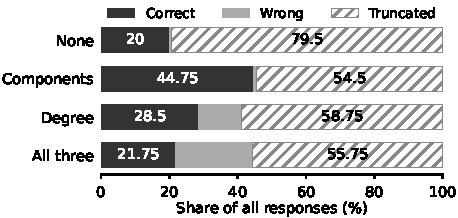
\includegraphics[width=\columnwidth]{edge_count_outcomes.pdf}
\caption{Thinking 4B on edge count: correct, wrong and truncated shares of \emph{all} responses. Conditions from top: none, components, degree, all three.}
\label{fig:outcomes}
\end{figure}

\paragraph{Thinking mode (\S\ref{sec:thinkmode}).} Thinking models check stated values against their own count. Under the degree primer, thinking 1.7B still lists the neighbors in $90\%$ of responses at $p\geq.35$; when their count conflicts with the stated value, thinking 1.7B and thinking 4B end on the stated value in $66\%$ and $93\%$ of cases. % [verify] [pdsource]
In the follow-ups, clustering gains thinking 1.7B $2.5$ points at $p\leq.50$ ($q=.043$) and loses $5.4$ at $p\geq.65$ ($q=.0015$), where filler loses $11.4$. % [ddthink]
Of the answers a condition changes, $44.4$--$64.5\%$ for thinking 1.7B and $83.3$--$95.2\%$ for thinking 4B involve a response that ran out of tokens; Figure~\ref{fig:outcomes} shows this for thinking 4B's edge count. % [churnwhy]

\paragraph{What responses rest on (\S\ref{sec:reston}).} Clustering and RWSE change the joint share with $q\geq.16$ in every arm. Plain 4B's is $85.75\%$ with no primer, $76.50\%$ with degree and $95.00\%$ with the component sentence; the degree primer raises plain 1.7B's from $54.00\%$ to $62.50\%$. % [joint]
Table~\ref{tab:cycles} classifies every correct, finished cycle-check answer by the argument it cites. For example, on one $p=.20$ graph plain 1.7B without a primer answers with $0\to4\to1\to5\to14\to13\to15\to16\to18\to\cdots\to38\to39\to0$, which climbs the ids almost in order; steps such as $15\to16$, $21\to25$ and $38\to39$ are not edges. % example: cycle_claims.csv, cycle_check/size40/p0.2/95
With thinking and no primer, valid arguments back $78.0\%$ and $95.8\%$ of all prompts. The degree primer raises plain 4B's valid share from $58.5\%$ to $76.5\%$. Truncation accounts for $21.2$ of the $21.8$ points it costs thinking 1.7B but only $8.2$ of the $17.5$ it costs plain 1.7B (Tables~\ref{tab:full} and~\ref{tab:truncmatrix}). RWSE, all three statistics and filler lower plain 4B's valid share to $33.2\%$, $45.2\%$ and $45.8\%$ ($q<.05$). % [ccvalid] [main] [trunc]

\paragraph{Node count.} The encoding's first line lists the $40$ node ids, so node count measures which number a model writes, not reading. Plain 1.7B answers $39$, the last id, on $68.5\%$ of finished responses without a primer and on $1.2\%$ under clustering, hence Table~\ref{tab:full}'s large node-count effects. % [nodecount] [ncanswer]

\section{Pilot and the Clustering Screen}
\label{app:pilot}
\paragraph{Pilot.} On the published GraphQA graphs ($5$--$19$ nodes), Gemma~4 E4B/12B and Qwen3-8B/14B, each in plain and thinking mode, were near ceiling without a primer on most tasks; only edge count separated them. This is why the main study uses 40-node graphs and smaller models.

\paragraph{The clustering effect.} Clustering on plain 1.7B's node degree emerged from a $40$-cell screen, so Table~\ref{tab:clust} tests it on graphs the screen did not see, on a fresh seed, against filler, on $20$--$160$-node graphs at fixed mean degree, at high density and on Qwen3-8B. The gain holds on unscreened graphs and on the fresh seed at low density, but not at high density or for Qwen3-8B. No response mentions clustering, and the gain does not depend on the queried node's printed coefficient ($p=.5$); it appears in how the response handles the node list. % [rqbehaviour] [rqhetero] [rqselection] [ddrep] [fixdeg8]
It falls on queried nodes early in the node list: $+5.01$, $+0.75$ and $-0.11$ points over the first, middle and last third at all seven densities, and $1.74$ points less per $10$ positions after adjusting for degree, clustering and density ($p=.018$); filler and components show no such gradient. It fixes $224$ copying errors in the neighbor list and introduces $176$. % [rqhetero] [rqbehaviour]
Components and filler also cut the neighbors the model misses ($0.94$ and $1.05$ per response at $p=.35$--$.50$, against $0.86$ with clustering and $1.49$ with none). % [rqbehaviour] [rqhetero]

\begin{table}[!t]
\centering\scriptsize
\setlength{\tabcolsep}{4pt}
\begin{tabular}{lrl}
\toprule
Test & Gain & $p$ or $q$\\
\midrule
Screened graphs ($700$) & $+1.29$ & $p=.47$\\ % [ddplain] [ddrep] [rqselection] [ddplainfill] [fixdeg8]
Unscreened graphs ($2{,}100$) & $+2.1$ & $p=.031$\\ % [ddplain] [ddrep] [rqselection] [ddplainfill] [fixdeg8]
$p\leq.50$ ($1{,}600$ pairs) & $+3.8$ & $q=.0035$\\ % [ddplain] [ddrep] [rqselection] [ddplainfill] [fixdeg8]
Fresh seed & $+4.2$ & $p=.00055$ ($.022$ corr.)\\ % [ddplain] [ddrep] [rqselection] [ddplainfill] [fixdeg8]
Against filler & $+3.2$ & $q=.014$\\ % [ddplain] [ddrep] [rqselection] [ddplainfill] [fixdeg8]
Fixed mean degree ($3{,}200$) & $+6.2$ & $q<.001$\\ % [fixdeg17]
$p\geq.65$ ($1{,}200$ pairs) & $-0.7$ & $q=.57$\\ % [ddplain] [ddrep] [rqselection] [ddplainfill] [fixdeg8]
Qwen3-8B ($3{,}200$) & $-1.0$ & $q=.05$\\ % [ddplain] [ddrep] [rqselection] [ddplainfill] [fixdeg8]
\bottomrule
\end{tabular}
\caption{The clustering effect on node degree against no primer (against filler where the row says so), in points, for plain Qwen3-1.7B except the last row, which is Qwen3-8B. \emph{Screened}: graphs the screen also used; \emph{fixed mean degree}: the $20$--$160$-node grid. \emph{corr.}: Bonferroni over the screen's cells.}
\label{tab:clust}
\end{table}

\end{document}
